% fig_lp_bracket: the LP bracket for one follower knapsack.
% For every leader choice x the follower's LP value U(x) and its integer value
% Phi(x) satisfy Phi(x) <= U(x) <= Phi(x) + p_max (the LP optimum has at most
% one fractional item).  Hence  min_x U(x) - p_max <= OPT = min_x Phi(x) <= Phi(x^)
% where x^ (x-hat) minimises U.  Schematic numbers, consistent with the rule:
%   U   = 12, 10.5, 9.2, 11, 9.8, 13, 10.6   (min 9.2 at x^ = 3rd choice)
%   Phi = 10,  9,   8,   9,  7,  11,  9      (OPT = 7)
%   p_max = 3, so the bracket is [6.2, 8] and contains 7.
% Build: pdflatex fig_lp_bracket.tex   (3.15 in x 1.6 in)
\documentclass[tikz,border=2pt]{standalone}
\pdfinfoomitdate=1 \pdftrailerid{} \pdfsuppressptexinfo=-1 % byte-identical rebuilds
\usepackage{mathptmx}
\usetikzlibrary{arrows.meta,calc,decorations.pathreplacing}
\definecolor{leader}{HTML}{2A78D6}
\definecolor{follower}{HTML}{EB6834}
\definecolor{cert}{HTML}{1BAF7A}
\definecolor{ink}{HTML}{0B0B0B}
\definecolor{ink2}{HTML}{52514E}
\definecolor{muted}{HTML}{A9A8A2}
\definecolor{grid}{HTML}{E6E5E0}
\tikzset{
  every picture/.style={font=\fontsize{8}{9.6}\selectfont, color=ink, line cap=round},
  small/.style={font=\fontsize{7}{8.4}\selectfont},
  lp/.style={draw=follower, fill=white, line width=0.8pt},
  ip/.style={fill=follower},
}
\begin{document}
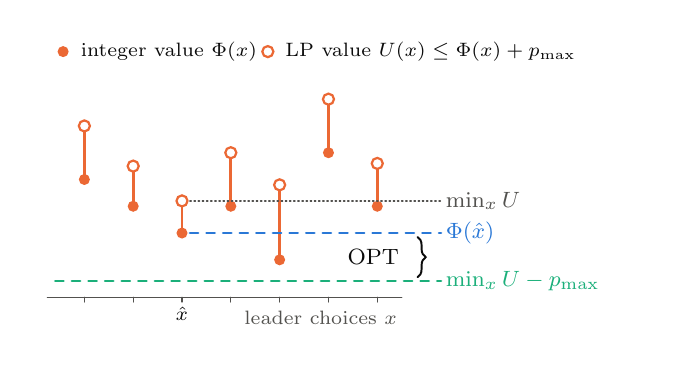
\begin{tikzpicture}
  % fixed page: 3.15 in x 1.6 in including the 2 pt border
  \useasboundingbox (0,0) rectangle (7.86,3.924);

  % axis of leader choices
  \draw[ink2, line width=0.5pt] (0.25,0.50) -- (4.75,0.50);
  \node[small, text=ink2, anchor=north east, inner sep=1.5pt] at (4.75,0.38) {leader choices $x$};

  % one bar per choice: Phi(x) (filled) up to U(x) (open)
  \foreach \i/\u/\p in {1/12/10, 2/10.5/9, 3/9.2/8, 4/11/9, 5/9.8/7, 6/13/11, 7/10.6/9}{
    \pgfmathsetmacro{\xx}{0.1+0.62*\i}
    \draw[ink2, line width=0.4pt] (\xx,0.50) -- ++(0,-0.06);
    \draw[follower, line width=1.0pt] (\xx,{0.50+(\p-5.6)*0.34}) -- (\xx,{0.50+(\u-5.6)*0.34});
    \fill[follower] (\xx,{0.50+(\p-5.6)*0.34}) circle (2.0pt);
    \draw[lp] (\xx,{0.50+(\u-5.6)*0.34}) circle (2.0pt);
  }
  \node[small, anchor=north, inner sep=1pt] at (0.1+0.62*3,0.42) {$\hat x$};

  % reference lines across the plot
  % min U (dotted grey), Phi(x^) (blue: the leader's point), min U - p_max (aqua: bound)
  \draw[ink2, line width=0.5pt, densely dotted] (2.06,{0.50+(9.2-5.6)*0.34}) -- (5.25,{0.50+(9.2-5.6)*0.34});
  \draw[leader, line width=0.9pt, dashed] (2.06,{0.50+(8-5.6)*0.34}) -- (5.25,{0.50+(8-5.6)*0.34});
  \draw[cert, line width=0.9pt, dashed] (0.35,{0.50+(6.2-5.6)*0.34}) -- (5.25,{0.50+(6.2-5.6)*0.34});
  \node[anchor=west, inner sep=1.5pt, text=ink2] at (5.25,{0.50+(9.2-5.6)*0.34}) {$\min_x U$};
  \node[anchor=west, inner sep=1.5pt, text=leader] at (5.25,{0.50+(8-5.6)*0.34}) {$\Phi(\hat x)$};
  \node[anchor=west, inner sep=1.5pt, text=cert] at (5.25,{0.50+(6.2-5.6)*0.34}) {$\min_x U - p_{\max}$};
  % the bracket that holds OPT
  \draw[decorate, decoration={brace, amplitude=3pt, mirror}, line width=0.7pt]
    (4.95,{0.50+(6.2-5.6)*0.34+0.05}) -- (4.95,{0.50+(8-5.6)*0.34-0.05})
    node[midway, anchor=east, xshift=-3pt] {OPT};

  % key
  \fill[follower] (0.45,3.62) circle (2.0pt);
  \node[small, anchor=west] at (0.55,3.62) {integer value $\Phi(x)$};
  \draw[lp] (3.05,3.62) circle (2.0pt);
  \node[small, anchor=west] at (3.15,3.62) {LP value $U(x) \le \Phi(x) + p_{\max}$};
\end{tikzpicture}
\end{document}
